%%
%% AgentTelemetry: Unified Observability for Autonomous AI Agent Systems
%% EuroMLSys 2026 — 6 pages (excl. bibliography) + appendix
%%

\documentclass[sigplan,10pt,screen]{acmart}

%% ---------- packages ----------
\usepackage{listings}
\usepackage{xcolor}
\usepackage{booktabs}
\usepackage{enumitem}
\usepackage{url}
\let\Bbbk\relax
\usepackage{amssymb}
\usepackage{tikz}
\usetikzlibrary{positioning,arrows.meta,fit,backgrounds}

%% ---------- listings style ----------
\lstset{
  language=Python,
  basicstyle=\ttfamily\scriptsize,
  keywordstyle=\color{blue!70!black}\bfseries,
  commentstyle=\color{green!50!black},
  stringstyle=\color{red!60!black},
  showstringspaces=false,
  breaklines=true,
  breakatwhitespace=true,
  frame=single,
  framesep=2pt,
  xleftmargin=4pt,
  xrightmargin=2pt,
  numbers=left,
  numberstyle=\tiny\color{gray},
  numbersep=4pt,
  aboveskip=6pt,
  belowskip=4pt,
  columns=flexible,
}

%% ---------- metadata ----------
\title{AgentTelemetry: Unified Observability for Autonomous AI Agent Systems}

\author{Krishna Chaitanya Balusu}
\affiliation{%
  \institution{Independent Researcher}
  \country{United States}
}
\email{krishnabkc15@gmail.com}

\begin{abstract}
Autonomous AI agents built on large language models are transitioning
from research prototypes to production deployments, yet observability
infrastructure for these systems remains fundamentally inadequate.
Standards such as OpenTelemetry lack semantic primitives for agent-specific
phenomena including reasoning chains, tool invocations, inter-agent
delegation, and cost accumulation.  We present \textsc{AgentTelemetry},
an open-source observability library that introduces (1)~a telemetry
data model with nine agent-specific span kinds and semantic attribute
conventions; (2)~W3C-compatible context propagation for multi-agent
tracing; (3)~a privacy-first design with opt-in content capture; and
(4)~a pluggable instrumentor--exporter architecture supporting seven
major agent frameworks with export to any OTLP backend.
Micro-benchmarks show instrumentation overhead under 13\,$\mu$s per
span ($<$0.003\% of typical LLM latency), and real-agent experiments
with Claude confirm suitability for always-on deployment.
\end{abstract}

\begin{CCSXML}
<ccs2012>
<concept>
<concept_id>10011007.10011074.10011099</concept_id>
<concept_desc>Software and its engineering~Software verification and validation</concept_desc>
<concept_significance>500</concept_significance>
</concept>
<concept>
<concept_id>10011007.10011074.10011111</concept_id>
<concept_desc>Software and its engineering~Software post-development issues</concept_desc>
<concept_significance>300</concept_significance>
</concept>
</ccs2012>
\end{CCSXML}

\ccsdesc[500]{Software and its engineering~Software verification and validation}
\ccsdesc[300]{Software and its engineering~Software post-development issues}

\keywords{AI agents, observability, telemetry, distributed tracing, LLM monitoring, OpenTelemetry, multi-agent systems}

\begin{document}

\maketitle

%% ====================================================================
%% 1. INTRODUCTION
%% ====================================================================
\section{Introduction}
\label{sec:introduction}

Large language model (LLM) based autonomous agents represent a paradigm shift
in software architecture.  Unlike conventional services that execute
deterministic logic, an LLM agent pursues a goal through iterative reasoning,
planning, tool use, and self-reflection---often delegating sub-tasks to other
agents~\cite{agentbench,agentboard}.  Frameworks such as LangChain, CrewAI,
AutoGen, and DSPy have accelerated adoption, and organizations are deploying
agents for customer support, code generation, and autonomous
operations~\cite{aiops_survey}.

This proliferation has exposed a critical gap: \emph{there is no
standardized observability infrastructure for AI agent systems}.
Production teams cannot reliably answer fundamental questions: Why did
the agent choose this tool?  Where did the hallucination originate?
How much did this task cost across all LLM calls?

OpenTelemetry (OTel)~\cite{otel} has become the standard for
distributed tracing in microservice architectures, but its
\texttt{Span\-Kind} enum and semantic conventions have no
representation for reasoning steps, LLM calls, tool invocations,
or inter-agent messages.

We present \textsc{AgentTelemetry}, an open-source library that fills
this gap.  Our contributions are:
\begin{enumerate}[leftmargin=*,nosep]
    \item A \textbf{telemetry data model} with nine agent-specific span
        kinds, semantic attribute conventions, and built-in cost estimation.
    \item A \textbf{context propagation protocol} compatible with W3C
        Trace Context, extended for multi-agent boundaries.
    \item A \textbf{privacy-first design} where prompt and completion
        content is never captured unless explicitly opted in.
    \item A \textbf{pluggable instrumentor--exporter architecture}
        with implementations for seven agent frameworks (LangChain,
        CrewAI, AutoGen, DSPy, Anthropic Claude, SmoLAgents,
        LlamaIndex) and three export targets including OTLP.
\end{enumerate}
\textsc{AgentTelemetry} is a \emph{production-oriented,
framework-agnostic telemetry library} that bridges existing distributed
tracing standards and the unique requirements of autonomous AI systems.

%% ====================================================================
%% 2. MOTIVATION AND GAP ANALYSIS
%% ====================================================================
\section{Motivation and Gap Analysis}
\label{sec:motivation}

An LLM agent's execution produces a deeply nested, non-deterministic trace
of cognitive operations.  A multi-agent research assistant---with planner,
researcher, and writer agents---may produce dozens of spans across three
or more agents, accumulating thousands of tokens and non-trivial cost.
Debugging a failure requires tracing backward across agent boundaries;
without unified tracing, operators resort to ad-hoc logging that is
inconsistent across frameworks and scales poorly.

OpenTelemetry provides trace and span identifiers, context propagation,
and a rich exporter ecosystem.  \textsc{AgentTelemetry} is designed to
be OTel-compatible, with spans mapping one-to-one to OTel spans via the
OTLP exporter.  However, OTel lacks the semantic layer needed for agent
observability.  Table~\ref{tab:gap} summarizes the gaps: OTel's
\texttt{SpanKind} has no equivalent for reasoning, planning, reflection,
or retrieval; its semantic conventions lack attributes for token counts,
model identity, cost, and agent role.

\begin{table}[t]
\centering
\small
\caption{Agent concepts mapped to observability primitives.  Bold entries
are novel \textsc{AgentTelemetry} contributions.}
\label{tab:gap}
\begin{tabular}{@{}lll@{}}
\toprule
\textbf{Agent Concept} & \textbf{OTel} & \textbf{AgentTelemetry} \\
\midrule
Agent            & Service         & \texttt{agent.name, .role} \\
Task execution   & Trace           & \textbf{AgentTrace} \\
Reasoning step   & (none)          & \textbf{REASONING span} \\
LLM call         & (none)          & \textbf{LLM\_CALL span} \\
Tool invocation  & (none)          & \textbf{TOOL\_CALL span} \\
Planning         & (none)          & \textbf{PLANNING span} \\
Self-reflection  & (none)          & \textbf{REFLECTION span} \\
Retrieval (RAG)  & (none)          & \textbf{RETRIEVAL span} \\
Agent message    & (none)          & \textbf{AGENT\_COMM span} \\
Human-in-loop    & (none)          & \textbf{HUMAN\_INPUT span} \\
Token count      & (none)          & \texttt{llm.input/output\_tokens} \\
Cost             & (none)          & \texttt{llm.cost\_usd} \\
\bottomrule
\end{tabular}
\end{table}

%% ====================================================================
%% 3. SYSTEM DESIGN
%% ====================================================================
\section{System Design}
\label{sec:design}

\textsc{AgentTelemetry} is organized into three layers: a core telemetry
model, a framework instrumentor layer, and an exporter layer.
Figure~\ref{fig:architecture} shows the architecture.

\begin{figure}[t]
\centering
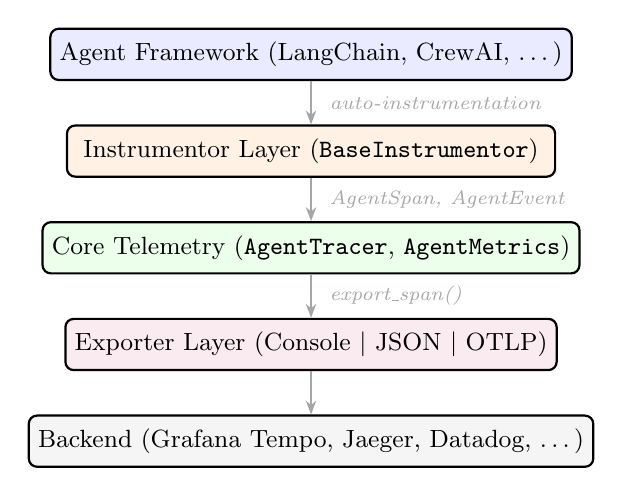
\begin{tikzpicture}[
    node distance=0.55cm,
    every node/.style={font=\small},
    layer/.style={draw, rounded corners=3pt, minimum width=6.2cm,
                  minimum height=0.65cm, align=center, thick},
    arrow/.style={-{Stealth[length=5pt]}, thick, gray!70},
    label/.style={font=\scriptsize\itshape, text=gray!70, anchor=west},
]
% Layers
\node[layer, fill=blue!8] (fw)
    {Agent Framework (LangChain, CrewAI, \ldots)};
\node[layer, fill=orange!10, below=of fw] (inst)
    {Instrumentor Layer (\texttt{BaseInstrumentor})};
\node[layer, fill=green!8, below=of inst] (core)
    {Core Telemetry (\texttt{AgentTracer}, \texttt{AgentMetrics})};
\node[layer, fill=purple!8, below=of core] (exp)
    {Exporter Layer (Console $|$ JSON $|$ OTLP)};
\node[layer, fill=gray!8, below=of exp] (back)
    {Backend (Grafana Tempo, Jaeger, Datadog, \ldots)};

% Arrows with labels
\draw[arrow] (fw) -- (inst) node[label, midway, right=3pt]
    {auto-instrumentation};
\draw[arrow] (inst) -- (core) node[label, midway, right=3pt]
    {AgentSpan, AgentEvent};
\draw[arrow] (core) -- (exp) node[label, midway, right=3pt]
    {export\_span()};
\draw[arrow] (exp) -- (back);
\end{tikzpicture}
\caption{Layered architecture of \textsc{AgentTelemetry}.  Instrumentors
are framework-specific; core and exporter layers are framework-agnostic.}
\label{fig:architecture}
\end{figure}

\subsection{Data Model and Span Kinds}
\label{sec:datamodel}

An \texttt{AgentSpan} encapsulates a unit of agent work, carrying a trace
identifier, span identifier, optional parent span, name, span kind, start
and end timestamps, terminal status, a set of semantic attributes, and an
ordered sequence of events.  The formal tuple definition and full span
lifecycle are provided in Appendix~\ref{app:datamodel}.

Spans progress through creation (ID allocation, timestamp), attribute
setting during execution, event recording for discrete occurrences, completion
with automatic cost estimation for \texttt{LLM\_CALL} spans, and export to
all registered backends.

The \texttt{AgentSpanKind} enumeration defines nine span types:
\texttt{TASK} (root), \texttt{REASONING} (chain-of-thought),
\texttt{LLM\_CALL} (model invocation), \texttt{TOOL\_CALL}
(function execution), \texttt{PLANNING} (task decomposition),
\texttt{REFLECTION} (self-critique), \texttt{RETRIEVAL} (RAG lookup),
\texttt{AGENT\_COMM} (inter-agent message), and \texttt{HUMAN\_INPUT}
(human-in-the-loop).  Each kind determines which semantic attributes are
expected (e.g., \texttt{LLM\_CALL} spans carry \texttt{llm.*} attributes)
and enables kind-specific dashboards and alerting.

We define three attribute namespaces: \texttt{agent.*} for identity
(name, framework, role), \texttt{llm.*} for model metadata (model,
tokens, cost, latency), and \texttt{tool.*} for tool execution (name,
input, output, success).  Cost is auto-estimated from model name and
token counts via a built-in pricing table.  Spans may contain timestamped
\texttt{AgentEvent} instances (e.g., \texttt{ERROR}, \texttt{WARNING},
\texttt{GUARDRAIL\_TRIGGERED}, \texttt{COST\_THRESHOLD}) for
fine-grained intra-span signals.  Full attribute tables are in
Appendix~\ref{app:datamodel}.

\subsection{Context Propagation and Privacy}
\label{sec:context}

Multi-agent architectures require trace context to flow across agent
boundaries.  The \texttt{AgentContext} class serializes context to a
carrier dictionary containing a W3C \texttt{traceparent} header, an
\texttt{agentstate} header with the source agent's name, and optional
\texttt{baggage} metadata.  The receiving agent deserializes the carrier
so that subsequent spans inherit the trace~ID and parent span reference,
producing a unified trace tree across multiple agents.

\textsc{AgentTelemetry} adopts a privacy-first posture: the
\texttt{llm.\allowbreak prompt} and \texttt{llm.\allowbreak completion}
attributes are \emph{never populated} unless the operator explicitly
sets \texttt{capture\_content=True}.  This opt-in gate applies at both
tracer and instrumentor levels.  When content capture is disabled,
telemetry still records all structural information---span kind,
duration, token counts, cost, model identity---providing comprehensive
observability without exposing sensitive content.

Complementing trace data, the \texttt{AgentMetrics} class provides
thread-safe counters, histograms, and gauges (see
Appendix~\ref{app:datamodel}).

%% ====================================================================
%% 4. IMPLEMENTATION
%% ====================================================================
\section{Implementation}
\label{sec:implementation}

\subsection{Instrumentor Architecture}
\label{sec:instrumentor}

The instrumentor layer uses a template method pattern.  The
abstract base instrumentor class provides a default tracer and
metrics instance, convenience methods for recording LLM and tool
metrics, abstract \texttt{instrument()} and \texttt{uninstrument()}
hooks for framework-specific patching, and a
\texttt{capture\_content} flag that propagates the privacy setting.
Listing~\ref{lst:usage} shows the usage pattern: the instrumentor
applies patches transparently and telemetry is collected without
changes to user code.

\begin{lstlisting}[caption={Instrumentor usage: automatic telemetry
  requires no user code changes.},
  label={lst:usage},float=t]
from agenttelemetry.instrumentors.langchain \
    import LangChainInstrumentor
from agenttelemetry.exporters.otlp \
    import OTLPExporter
inst = LangChainInstrumentor()
inst.tracer.add_exporter(
    OTLPExporter(endpoint="collector:4317"))
inst.instrument()
agent = create_langchain_agent(...)
result = agent.invoke("Summarize this paper")
inst.uninstrument()
\end{lstlisting}

Three exporters are provided: a console exporter for development
(single-line span summaries), a JSON file exporter for offline
analysis (JSON Lines format), and an OTLP exporter for production
backends via gRPC.  The exporter interface is a single
\texttt{export\_span()} method, making custom exporters
straightforward.  Pre-built Grafana dashboards for agent overview
and trace detail are included (Appendix~\ref{app:dashboards}).

The direct tracing API (\texttt{AgentTracer}) provides context-manager
methods for each span kind, enabling manual instrumentation of custom
agent implementations (see Appendix~\ref{app:tracing_api}).

\subsection{Framework Support}
\label{sec:frameworks}

We provide instrumentors for seven major agent frameworks.
Table~\ref{tab:framework_comparison} summarizes which agent concepts
each framework natively exposes and how \textsc{AgentTelemetry} maps
them to spans.

\begin{table}[t]
\centering
\scriptsize
\caption{Framework support: agent concepts exposed by each framework
and mapping to \textsc{AgentTelemetry} span kinds.  \checkmark\,=
auto-instrumented; ---\,= not natively present.}
\label{tab:framework_comparison}
\begin{tabular}{@{}lccccccc@{}}
\toprule
\textbf{Concept} & \rotatebox{70}{\textbf{LangChain}} &
\rotatebox{70}{\textbf{CrewAI}} & \rotatebox{70}{\textbf{AutoGen}} &
\rotatebox{70}{\textbf{DSPy}} & \rotatebox{70}{\textbf{Claude}} &
\rotatebox{70}{\textbf{SmoLAgents}} & \rotatebox{70}{\textbf{LlamaIndex}} \\
\midrule
Task root    & \checkmark & \checkmark & ---        & \checkmark & \checkmark & \checkmark & \checkmark \\
LLM call     & \checkmark & \checkmark & \checkmark & \checkmark & \checkmark & \checkmark & \checkmark \\
Tool call    & \checkmark & ---        & \checkmark & ---        & \checkmark & \checkmark & \checkmark \\
Reasoning    & \checkmark & \checkmark & \checkmark & \checkmark & \checkmark & \checkmark & --- \\
Retrieval    & \checkmark & ---        & ---        & \checkmark & ---        & ---        & \checkmark \\
Agent comm   & ---        & \checkmark & \checkmark & ---        & ---        & ---        & --- \\
Token count  & \checkmark & \checkmark & \checkmark & \checkmark & \checkmark & \checkmark & \checkmark \\
Cost track   & ---        & \checkmark & ---        & ---        & \checkmark & ---        & --- \\
\bottomrule
\end{tabular}
\end{table}

No single framework exposes all nine agent concepts.  LangChain covers
LLM calls, tools, and retrieval but lacks inter-agent communication;
CrewAI provides multi-agent delegation but omits tool calls; AutoGen
captures messaging and tools but has no task root; the Anthropic Claude
instrumentor captures tool use blocks and extended thinking; SmoLAgents
tracks code agent steps; and LlamaIndex provides deep query engine and
retriever integration.  \textsc{AgentTelemetry}'s uniform span vocabulary
enables cross-framework consistency: dashboards built for one framework
work identically for another.

%% ====================================================================
%% 5. EVALUATION
%% ====================================================================
\section{Evaluation}
\label{sec:evaluation}

\subsection{Instrumentation Overhead}
\label{sec:overhead}

We measured per-operation overhead on Apple Silicon (macOS~25.2,
Python~3.9.6) over five independent trials of 10{,}000 iterations
each.  Table~\ref{tab:overhead} presents the results.

\begin{table}[t]
\centering
\small
\caption{Per-operation overhead (10{,}000~ops, 5~trials, mean~$\pm$~std).}
\label{tab:overhead}
\begin{tabular}{@{}lr@{~$\pm$~}r@{}}
\toprule
\textbf{Operation} & \multicolumn{2}{c}{\textbf{Latency ($\mu$s/op)}} \\
\midrule
Span creation (bare)           & 12.15 & 0.07 \\
Span creation (w/ attributes)  & 12.57 & 0.05 \\
Context propagation (round-trip) & 1.45 & 0.01 \\
ConsoleExporter (to \texttt{/dev/null})  & 1.54 & 0.03 \\
JSONFileExporter (to temp file) & 103.48 & 6.29 \\
Nested trace (4-deep)          & 28.95 & 0.14 \\
Cost estimation                &  0.35 & 0.00 \\
\bottomrule
\end{tabular}
\end{table}

Span creation costs $\sim$12\,$\mu$s, with negligible overhead for
attributes.  A four-level nested trace (task $\to$ reasoning $\to$
LLM call $\to$ tool call) costs $\sim$29\,$\mu$s total.  Context
propagation adds 1.45\,$\mu$s per round trip.  Since LLM API calls
take 500\,ms--5\,s, the most expensive in-memory operation (span
creation) represents $<$0.003\% overhead, confirming suitability for
always-on production deployment.

\subsection{Real-Agent Experiment}
\label{sec:real_agent}

To validate instrumentation on real workloads, we ran a tool-calling
agent using the Anthropic SDK (Claude Sonnet~4) instrumented with
\textsc{AgentTelemetry}'s \texttt{Claude\-Agent\-Instrumentor} against
an uninstrumented baseline.  The agent performed a multi-step
question-answering task requiring two tools (search and calculator),
executing an agentic loop of LLM calls and tool invocations.  We
measured end-to-end latency over 10 runs per condition and captured
traces via \texttt{JSON\-File\-Exporter}.

The instrumented agent produced 5 spans per invocation (3
\texttt{LLM\_CALL}, 2 \texttt{TOOL\_CALL}), automatically capturing
token counts ($\sim$1{,}750 input, $\sim$180 output per run), cost
estimates (\$0.008/run), and tool success status.  Baseline latency
was 7{,}507$\pm$1{,}707\,ms; instrumented latency was
7{,}495$\pm$2{,}086\,ms---a difference of $-$13\,ms ($-$0.17\%),
well within measurement noise.  This confirms that instrumentation
overhead is negligible relative to LLM API latency, consistent with
our micro-benchmark results.

\subsection{Debugging Effectiveness}
\label{sec:case_study}

We evaluated fault diagnosis using a simulated multi-agent pipeline
(planner $\to$ researcher $\to$ writer) with three injected faults:
(1)~hallucinated retrieval (relevance score 0.12, threshold 0.5);
(2)~tool timeout with retry producing degraded results; and
(3)~cost overrun from an 8-iteration reasoning loop exceeding a
\$1.00 budget.  Table~\ref{tab:diagnosis} summarizes the results.

\begin{table}[t]
\centering
\small
\caption{Debugging effectiveness: default logging vs.\
\textsc{AgentTelemetry} across three fault scenarios.}
\label{tab:diagnosis}
\begin{tabular}{@{}lcc@{}}
\toprule
\textbf{Metric} & \textbf{Default} & \textbf{AgentTelemetry} \\
\midrule
\multicolumn{3}{@{}l}{\emph{S1: Hallucinated Retrieval}} \\
~~Root cause found   & Rarely     & Always \\
~~Cross-agent tracing & Manual    & Automatic \\
\midrule
\multicolumn{3}{@{}l}{\emph{S2: Tool Timeout}} \\
~~Causal chain visible  & Partial & Complete \\
~~Retry context captured & No     & Yes \\
\midrule
\multicolumn{3}{@{}l}{\emph{S3: Cost Overrun}} \\
~~Per-iteration cost   & Unavailable & Tracked \\
~~Threshold event      & None        & Automatic \\
\bottomrule
\end{tabular}
\end{table}

Agent-specific span kinds (\texttt{RETRIEVAL}, \texttt{TOOL\_\allowbreak CALL},
\texttt{LLM\_\allowbreak CALL}, \texttt{REASONING}) combined with
semantic attributes (relevance scores, cost accumulators) and
structured events (\texttt{WARNING}, \texttt{COST\_\allowbreak THRESHOLD})
enable rapid root-cause diagnosis that is impractical with generic
logging.  Cross-agent fault propagation and per-iteration cost
attribution are fundamentally impossible without structured
multi-agent telemetry.

\subsection{Threats to Validity}
\label{sec:threats}

Our evaluation has several limitations.  The micro-benchmarks were
conducted on a single machine (Apple Silicon); overhead may vary on
different architectures.  The real-agent experiment uses a single
framework (Anthropic Claude SDK); while the instrumentor architecture
is framework-agnostic, overhead characteristics may differ across
frameworks.  The debugging case study uses simulated fault injection
with controlled latencies rather than production failures.  We did not
evaluate multi-machine distributed tracing, though the W3C-compatible
context propagation is designed for this scenario.

%% ====================================================================
%% 6. RELATED WORK
%% ====================================================================
\section{Related Work}
\label{sec:related}

\paragraph{System-Level Agent Monitoring.}
AgentSight~\cite{agentsight} uses eBPF to monitor TLS-encrypted LLM
traffic and correlate kernel events with agent intent.  While it provides
deep system-level visibility, it requires Linux kernel access often
unavailable in containers and cannot capture application-level semantics
(agent role, task decomposition).  \textsc{AgentTelemetry} operates at
the application level; the two approaches are complementary.

\paragraph{Runtime Safety and Constraints.}
NeMo Guardrails~\cite{nemo_guardrails} intercepts and validates agent
behavior; DSPy Assertions~\cite{dspy_assertions} embed constraints into
LLM pipelines.  Both enforce policies but do not produce structured,
exportable telemetry for dashboards or SLO monitoring.

\paragraph{Agent Evaluation.}
AgentBench~\cite{agentbench}, AgentBoard~\cite{agentboard}, and
Agent-as-a-Judge~\cite{agent_as_judge} target offline evaluation, not
continuous production monitoring.

\paragraph{Commercial Platforms.}
LangSmith~\cite{langsmith} provides tracing for LangChain but is
ecosystem-specific and proprietary.
OpenLLMetry~\cite{openllmetry} extends OTel with LLM instrumentation
but focuses on individual API calls without agent-level abstractions
(task, reasoning, inter-agent communication).
\textsc{AgentTelemetry} is fully open-source, framework-agnostic,
standards-based (OTLP), and provides nine agent-specific span kinds
that capture the full complexity of multi-agent systems.

%% ====================================================================
%% 7. CONCLUSION
%% ====================================================================
\section{Conclusion}
\label{sec:conclusion}

We have presented \textsc{AgentTelemetry}, an open-source framework
for unified observability of autonomous AI agent systems.  By
introducing agent-specific span kinds, semantic conventions,
W3C-compatible context propagation, and privacy-first design, it
bridges the gap between distributed tracing standards and LLM-based
agent workloads.  Its instrumentor--exporter architecture supports
seven frameworks with export to any OTLP backend.

Future directions include proposing our semantic conventions as
an OpenTelemetry Enhancement Proposal~(OTEP), adaptive sampling
that retains anomalous traces~\cite{sieve_sampling}, real-time
span streaming for long-running tasks, and applying causal
inference~\cite{mulan} to automated root cause analysis.

%% ====================================================================
%% BIBLIOGRAPHY
%% ====================================================================

\begin{thebibliography}{20}

\bibitem{agentsight}
Y.~Zheng, Y.~Hu, T.~Yu, and A.~Quinn.
\newblock {AgentSight}: System-Level Observability for {AI} Agents Using {eBPF}.
\newblock {\em arXiv preprint arXiv:2508.02736}, 2025.

\bibitem{nemo_guardrails}
T.~Rebedea, R.~Dinu, M.~Sreedhar, C.~Parisien, and J.~Cohen.
\newblock {NeMo Guardrails}: A Toolkit for Controllable and Safe {LLM}
  Applications.
\newblock In {\em Proc.\ EMNLP (Demo Track)}, 2023.

\bibitem{dspy_assertions}
A.~Singhvi, M.~Shetty, S.~Tan, C.~Potts, K.~Sen, M.~Zaharia, and O.~Khattab.
\newblock {DSPy} Assertions: Computational Constraints for Self-Refining
  Language Model Pipelines.
\newblock In {\em Proc.\ COLM}, 2024.

\bibitem{agentboard}
C.~Ma, J.~Zhang, Z.~Zhu, C.~Yang, Y.~Yang, et~al.
\newblock {AgentBoard}: An Analytical Evaluation Board of Multi-Turn {LLM}
  Agents.
\newblock In {\em Proc.\ ACL}, 2024.

\bibitem{agent_as_judge}
M.~Zhuge, C.~Zhao, D.~Ashley, et~al.
\newblock Agent-as-a-Judge: Evaluate Agents with Agents.
\newblock {\em arXiv preprint arXiv:2410.10934}, 2024.

\bibitem{agentbench}
X.~Liu, H.~Yu, H.~Zhang, et~al.
\newblock {AgentBench}: Evaluating {LLMs} as Agents.
\newblock In {\em Proc.\ ICLR}, 2024.

\bibitem{openagentsafety}
S.~Vijayvargiya, A.~B.~Soni, X.~Zhou, Z.~Z.~Wang, N.~Dziri, G.~Neubig, and
  M.~Sap.
\newblock {OpenAgentSafety}: A Comprehensive Framework for Evaluating
  Real-World {AI} Agent Safety.
\newblock {\em arXiv preprint arXiv:2507.06134}, 2025.

\bibitem{toolemu}
Y.~Ruan, H.~Dong, A.~Wang, S.~Pitis, et~al.
\newblock {ToolEmu}: Identifying Risks of {LLM} Agents with an {LLM}-Emulated
  Sandbox.
\newblock In {\em Proc.\ ICLR}, 2024.

\bibitem{ml_monitoring}
J.~Leest, I.~Gerostathopoulos, P.~Lago, and C.~Raibulet.
\newblock Monitoring and Observability of Machine Learning Systems: Current
  Practices and Gaps.
\newblock {\em arXiv preprint arXiv:2510.24142}, 2025.

\bibitem{aiops_survey}
L.~Zhang, T.~Jia, M.~Jia, Y.~Wu, A.~Liu, Y.~Yang, Z.~Wu, X.~Hu, P.~S.~Yu,
  and Y.~Li.
\newblock A Survey of {AIOps} in the Era of Large Language Models.
\newblock {\em arXiv preprint arXiv:2507.12472}, 2025.

\bibitem{otel}
{OpenTelemetry Authors}.
\newblock {OpenTelemetry Specification}, v1.30.
\newblock \url{https://opentelemetry.io/docs/specs/otel/}, 2024.

\bibitem{tracediag}
R.~Ding, C.~Zhang, L.~Wang, Y.~Xu, M.~Ma, W.~Zhang, S.~Qin, S.~Rajmohan,
  Q.~Lin, and D.~Zhang.
\newblock {TraceDiag}: Adaptive, Interpretable, and Efficient Root Cause
  Analysis on Large-Scale Microservice Systems.
\newblock In {\em Proc.\ ACM ESEC/FSE}, 2023.

\bibitem{deeptralog}
C.~Zhang, X.~Peng, C.~Sha, K.~Zhang, Z.~Fu, X.~Wu, Q.~Lin, and D.~Zhang.
\newblock {DeepTraLog}: Trace-Log Combined Microservice Anomaly Detection
  through Graph-based Deep Learning.
\newblock In {\em Proc.\ ACM ICSE}, 2022.

\bibitem{sieve_sampling}
D.~Batavia, I.~Weber, et~al.
\newblock {Sieve}: Attention-based Sampling of End-to-End Trace Data in
  Distributed Microservice Systems.
\newblock In {\em Proc.\ IEEE ICWS}, 2023.

\bibitem{mulan}
L.~Zheng, Z.~Chen, J.~He, and H.~Chen.
\newblock {MULAN}: Multi-modal Causal Structure Learning for Root Cause
  Analysis.
\newblock In {\em Proc.\ NeurIPS}, 2024.

\bibitem{langsmith}
{LangChain Inc.}
\newblock {LangSmith}: Platform for Building Production-Grade {LLM} Applications.
\newblock \url{https://smith.langchain.com/}, 2024.

\bibitem{openllmetry}
{Traceloop}.
\newblock {OpenLLMetry}: Open-Source Observability for {LLM} Applications
  Built on {OpenTelemetry}.
\newblock \url{https://github.com/traceloop/openllmetry}, 2024.

\end{thebibliography}

%% ====================================================================
%% APPENDICES (unlimited, after bibliography)
%% ====================================================================

\appendix

\section{Formal Data Model}
\label{app:datamodel}

\paragraph{Formal Definition.}
We define an \texttt{AgentSpan} as a tuple:
\[
  s = (t, s_{\mathrm{id}}, p_{\mathrm{id}}, \mathit{name}, k, t_0, t_1, \sigma, A, E)
\]
where $t \in \{0,1\}^{128}$ is the trace identifier, $s_{\mathrm{id}} \in \{0,1\}^{64}$ is the span identifier, $p_{\mathrm{id}} \in \{0,1\}^{64} \cup \{\bot\}$ is the optional parent span identifier, $\mathit{name}$ is a human-readable label, $k \in \mathcal{K}$ is the span kind drawn from the \texttt{AgentSpanKind} enumeration, $t_0$ and $t_1$ are nanosecond-precision timestamps, $\sigma \in \{\texttt{UNSET}, \texttt{OK}, \texttt{ERROR}, \texttt{TIMEOUT}\}$ is the terminal status, $A : \mathit{String} \rightharpoonup \mathit{Value}$ is a partial function mapping attribute keys to values, and $E$ is an ordered sequence of \texttt{AgentEvent} instances.

\paragraph{Span Lifecycle.}
An \texttt{AgentSpan} progresses through five phases:
\begin{enumerate}[leftmargin=*,nosep]
    \item \textbf{Creation.}  The tracer allocates the span, assigns $s_{\mathrm{id}}$, inherits $t$ and $p_{\mathrm{id}}$ from the active span stack, and records $t_0 = \mathit{now}()$.
    \item \textbf{Attribute Setting.}  The caller attaches metadata via \texttt{set\_attribute(key, value)}.  Attributes are additive and last-writer-wins.
    \item \textbf{Event Recording.}  Discrete occurrences (errors, guardrail triggers, cost thresholds) are captured via \texttt{add\_event()}.
    \item \textbf{Completion.}  The context manager records $t_1$ and promotes $\sigma$ to \texttt{OK} if still \texttt{UNSET}.  For \texttt{LLM\_CALL} spans, cost is auto-estimated.
    \item \textbf{Export.}  The span is serialized and dispatched to all registered exporters.
\end{enumerate}

\paragraph{Semantic Attribute Conventions.}
Three attribute namespaces are defined:

\begin{description}[leftmargin=*,nosep,style=unboxed]
    \item[\texttt{agent.*}] Agent identity: \texttt{agent.name}, \texttt{agent.framework}, \texttt{agent.framework.version}, \texttt{agent.role}, \texttt{agent.task}.
    \item[\texttt{llm.*}] LLM metadata: \texttt{llm.model}, \texttt{llm.provider}, \texttt{llm.input\_tokens}, \texttt{llm.output\_tokens}, \texttt{llm.total\_tokens}, \texttt{llm.temperature}, \texttt{llm.cost\_usd}, \texttt{llm.latency\_ms}.
    \item[\texttt{tool.*}] Tool execution: \texttt{tool.name}, \texttt{tool.description}, \texttt{tool.input}, \texttt{tool.output}, \texttt{tool.success}, \texttt{tool.error}, \texttt{tool.latency\_ms}.
\end{description}

\paragraph{Events.}
Spans can contain timestamped \texttt{AgentEvent} instances categorized by \texttt{EventType}: \texttt{LLM\_START}, \texttt{LLM\_END}, \texttt{TOOL\_START}, \texttt{TOOL\_END}, \texttt{GUARDRAIL\_TRIGGERED}, \texttt{COST\_THRESHOLD}, \texttt{ERROR}, \texttt{WARNING}, and others.

\paragraph{Metrics.}
The \texttt{AgentMetrics} class provides thread-safe counters (e.g., \texttt{agent.llm.call.count}, \texttt{agent.cost.total\_usd}), histograms (e.g., \texttt{agent.llm.latency\_ms}), and gauges.  The \texttt{summary()} method computes descriptive statistics (min, max, mean, p50, p95, p99).

\section{Tracing API}
\label{app:tracing_api}

The \texttt{AgentTracer} class provides context-manager methods for each span kind.  The following listing illustrates direct API usage for custom agent implementations:

\begin{lstlisting}[caption={Direct tracing API for custom agents.}]
tracer = AgentTracer(
    agent_name="researcher",
    framework="custom",
    capture_content=False)
tracer.add_exporter(ConsoleExporter())
with tracer.start_task("Analyze dataset") as t:
  with tracer.start_planning("decompose") as p:
    pass  # planning logic
  with tracer.start_llm_call(model="gpt-4o") as l:
    l.set_attribute("llm.input_tokens", 1200)
    l.set_attribute("llm.output_tokens", 450)
  with tracer.start_tool_call("sql_query") as tc:
    tc.set_attribute("tool.input", "SELECT ...")
    tc.set_attribute("tool.success", True)
\end{lstlisting}

\section{Grafana Dashboard Integration}
\label{app:dashboards}

\textsc{AgentTelemetry} ships two pre-built Grafana dashboards for the OTLP export path, distributed as importable JSON models compatible with Grafana~10+.

\paragraph{Agent Overview Dashboard.}
The overview dashboard provides aggregate operational metrics: stat panels for Total Tasks, LLM Calls, Tool Calls, Cost (USD), and Active Agents; time-series panels for LLM Latency and Task Duration by agent; stacked bar charts for Token Usage by Model; and pie charts for Cost Breakdown by Model.

\paragraph{Agent Trace Detail Dashboard.}
The trace detail dashboard enables deep inspection of individual traces using Grafana Tempo, Prometheus, and Loki.  Panels include per-trace summary statistics, a span waterfall timeline, sortable span detail tables, LLM Call and Tool Call detail views, a node graph for multi-agent topology, and event/error log panels.

\section{Extended Case Study Narratives}
\label{app:casestudy}

\paragraph{Scenario 1: Hallucinated Retrieval.}
The researcher agent's RAG vector search returns documents with relevance score 0.12 (threshold 0.5).  The \textsc{AgentTelemetry} trace reveals the fault immediately: the \texttt{RETRIEVAL} span carries \texttt{retrieval.relevance\_score=0.12} and a \texttt{WARNING} event.  The downstream \texttt{LLM\_CALL} span shows \texttt{llm.context\_quality=degraded}.  Following the parent--child chain from the writer's \texttt{TASK} span back through the researcher to the \texttt{RETRIEVAL} span localizes the root cause.  Without structured telemetry, only the writer's incorrect output is visible, and diagnosis requires manual correlation across three agents' logs.

\paragraph{Scenario 2: Tool Timeout with Retry.}
A \texttt{web\_search} tool call times out after 30\,s; the researcher retries with a simplified query, receiving only 2 results instead of 10.  The trace shows: a \texttt{TOOL\_CALL} span with \texttt{status=ERROR} and \texttt{tool.error=TimeoutError}, a retry \texttt{WARNING} event, a second \texttt{TOOL\_CALL} with reduced results, and an \texttt{LLM\_CALL} with \texttt{context\_quality=degraded}.

\paragraph{Scenario 3: Cost Overrun.}
The researcher enters a self-critique loop iterating 8 times (expected 2--3), each iteration making an \texttt{LLM\_CALL} with growing token counts.  Each iteration is captured as a nested \texttt{REASONING} span with \texttt{reasoning.iteration} and \texttt{reasoning.cumulative\_cost\_usd} attributes.  A \texttt{COST\_THRESHOLD} event fires at the exact iteration where cost exceeds \$1.00.

\section{Extended Related Work}
\label{app:extended_related}

\paragraph{Agent Safety.}
ToolEmu~\cite{toolemu} emulates tool execution for automated safety testing.  OpenAgentSafety~\cite{openagentsafety} evaluates agent safety across 350+ tasks, finding unsafe behavior in over 51\% of safety-vulnerable tasks.  These findings underscore the need for runtime observability beyond development-time evaluation.

\paragraph{ML System Monitoring.}
Leest et al.~\cite{ml_monitoring} documented significant gaps in ML monitoring practice, motivating standardized tools for ML-specific observability.

\paragraph{AIOps and Distributed Tracing.}
TraceDiag~\cite{tracediag} and DeepTraLog~\cite{deeptralog} analyze distributed traces for fault diagnosis in microservices.  \textsc{AgentTelemetry}'s OTLP export enables these tools to be applied directly to agent telemetry data.

\end{document}
